\section{Implementation}
\label{sec-impl}

In \S \ref{sec-methods} the strategies and interfaces that \Cyclus uses to 
simplify archetype development were presented. These represent notions about
the amount of information and prior knowledge that the archetype developer 
must have in order to write archetypes.  If a particular particular strategy 
decreased the knowledge required by archetype developers then it is considered
easier and beneficial to implement.  

However, methods that are more inuitive for new users to understand are often
propotionatly more difficult to implement. For example, it is one thing to 
learn to play the game \emph{tic-tac-toe}, or even master it; it is quite another
thing to design the game \emph{tic-tac-toe} in the first place.  
A sublime interface belies 
herculean effort. This section descibes the infrastructre that holds up 
current \cyclus archetype development.  This is relevant to other fuel 
cycle simulators that wish to adopt the same strategies that \cyclus 
implements. In particular, the implemention of the \cyclus preprocessor, 
the type system, input file validation, metadata annotations will all 
be covered here.

\subsection{The \Cyclus Preprocessor}

The \cyclus preprocessor, \cycpp, is resposnible for all metadata collection and 
code generation for archetypes. It is implemented as a small Python utility 
currently less than 2000 lines in a single file.  It has no dependencies other 
than the Python standard library. It is thus light-weight enough to move around 
between code projects, if needed. For the scale of its responsibility, \cycpp
is extremely efficient. 

The preprocessor implements the three passes detailed in \S\ref{subsec-ppgc}:
normalization via standard \code{cpp}, state variable annotation accumulation, and code 
generation. The \cycpp tool must be run on all C++ header and source files that
contain archetype code and the \code{#pragma cyclus} directives. Running \cycpp
on files without such directives does no harm and will result in exactly the 
original file. The first \cycpp
pass, running the C preprocessor over these files, is a trivial subprocess 
spawn. The only potential trouble spots here are ensureing that \cycpp sees the
same include, macro defintitions, and macro undefinitions that actual compilation 
of the source code will have.

The second pass, state accumulation, represents half of the work that \cycpp performs.
The results from pass 1 is fed into this pass and scoured for 
potentially relevant information about the archetypes present in the file. 
Thus, state accumulation 
may be thought of as a traditional parser which tranforms tokens (line of the 
C++ file) into a more meaningful in-memory data structure. As a parser, pass 2 
may be implemented as a \emph{state machine} \cite{mertz2003text,wagner2006modeling}.

Pass 2 is represented in \cycpp by the \code{StateAccumulator} class.  This is a
state machine which takes lines output from the C preproessor and compares them 
against a seires of \emph{filters}.  If a line matches the expected structure 
for a filter, then the filter executes a \emph{transformation} function on the 
line and no further filters are executed. If the line does not match any filters
then the line is allowed to pass through the \code{StateAccumulator}. 
The filter-transformation sequence can be thought of in analogy to a sphere of a 
given radius (a line of code) attempting to pass through concentric windows 
(the filters) of decreasing appeture. This first window where the sphere stops 
represents the transformation that is executed.  This sphere is allowed to 
move through the system without being stopped. This analogy may be seen in 
Figure \ref{filter-analogy}.  

\begin{figure}[htbc]
\label{filter-analogy}
\centering
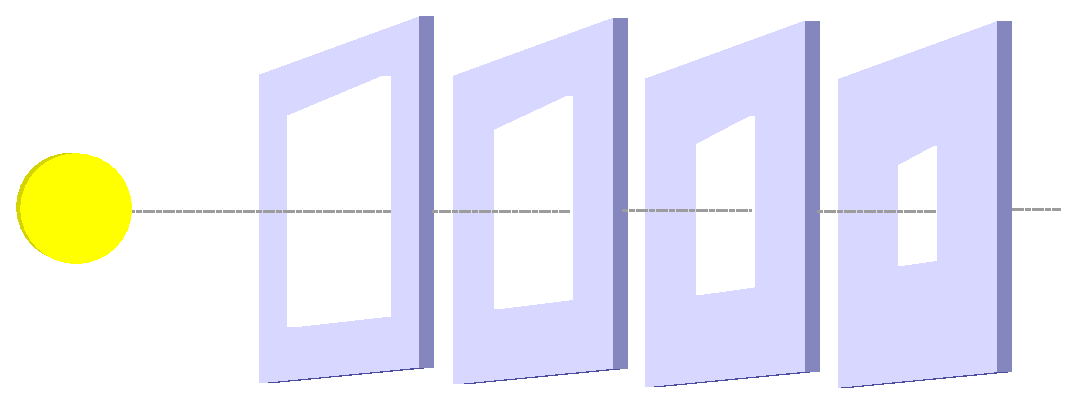
\includegraphics[width=0.8\textwidth]{filter-analogy.eps}
\caption{The \code{StateAccumulator} class passes lines of C++ code through 
a series of filters, each of which may transform the information heretofore gathered
by previous filters. 
This may be thought of analogous to a spheres of various radii rolling through 
concentric windows.  The spheres, or lines of code, stop rolling when they hit a  
window, or filter. This triggers the execution of the transformation function of just 
that filter and that filter alone.}
\end{figure}

The filters implemented for pass 2 of \cycpp are described in Table \ref{pass2-filters}, 
in order of decreasing precedence. The most importnat of these filters implement 
the \code{#pragma cyclus} dirctives that the archetype uses to communicate
with the preprocessor.  The pragma filters tend to modify attributes of
the \code{StateAccumulator} such as the \code{context}, the \code{execns} 
(or \emph{execution namespace}), the \code{aliases} set, and the \code{namespaces}. 
These represent the classes, types, aliases, and other information that defines
the scope of the C++ code that has been seen thusfar. Such information is necessary 
for accurately representing archetypes and their state variables. 

Most pass 2 filters that do not implement a preprocessor directive instead
aggregate information about the available types. The \code{VarDeclarationFilter} has
the important job of determining the C++ type of state variables from the 
member variable declaration on the archetype class. However, the C++ type system 
is a complex beast that allows for a number of programmer modifications prior 
to the type declarations.  Types may be aliased to any number of alternative 
names, template types are white-space insensitive, scoping rules apply 
to new type names, and other issues must be resolved to accurately and uniquely 
represent a C++ type.  This requires that \cycpp reimplement relevant type handling
simply to get the spellings correct. 
Thus the \code{StateAccumulator} accumulator acts as its own type system and is 
able to return the canonical form of any type it knows about at all points during 
pass 2 of \cycpp.

\begin{table}
\label{pass2-filters}
\caption{\cyclus Preprocessor Pass 2 Filters, higher order filters have 
         lower execution precedence.}
\begin{tabular}[htb]{|p{0.05\linewidth}|p{0.33\linewidth}|p{0.6\linewidth}|}
\hline
\textbf{order} & \textbf{filter} & \textbf{description} \\
\hline
1  & \code{ClassAndSuperclassFilter} & Accumultes the class name from a class 
                                       declaration. Also stores the names of the 
                                       superclasses from the declaration.\\ 
\hline
2  & \code{AccessFilter} & Sets the current access control level, either 
                           \code{public}, \code{private}, or \code{protected}.\\
\hline
3  & \code{ExecFilter} & Implements the \code{#pragma cyclus exec <code>} directive
                         that allows for the execution of arbitrary Python code.
                         The results of this code are added the context that 
                         evaluated other \cycpp directives.\\ 
\hline
4  & \code{UsingNamespaceFilter} & Adds and removes a namespace from the 
                                   current scope via the C++ \code{using namespace}
                                   statement.\\ 
\hline
5  & \code{NamespaceAliasFilter} & Implements namespace aliasing in the current 
                                   scope.\\ 
\hline
6  & \code{NamespaceFilter} & Sets and reverts a new namepsace scope.\\ 
\hline
7  & \code{TypedefFilter} & Adds a type alias to the current scope via the 
                            C++ \code{typedef} statement.\\ 
\hline
8  & \code{UsingFilter} & Removes scope from a type by adding an alias in the 
                          current scope via the C++ \code{using} statement.\\ 
\hline
9  & \code{LinemarkerFilter} & Interprets \code{cpp} linemarker dirctives in order
                               to produce more useful debugging information in 
                               \cycpp.\\ 
\hline
10 & \code{NoteDecorationFilter} & Handles the \cycpp \code{#pragma cyclus note <dict>}
                                   directive by evaluating the contents of 
                                   \code{<dict>} and adding them to the archetype 
                                   annotations.\\ 
\hline
11 & \code{VarDecorationFilter} & Implements the \cycpp \code{#pragma cyclus var <dict>}
                                  directive for state variable annotations. The 
                                  \code{<dict>} is evaluated in the current 
                                  context and queued up to be applied to the 
                                  next state variable declaration.\\ 
\hline
12 & \code{VarDeclarationFilter} & State variable declaration. Applies the results 
                                   of the immeadiately prior \code{VarDecorationFilter}
                                   as the state variable annotations. Furthermore, 
                                   this filter parses out the name of the 
                                   state variable, its index with respect to other 
                                   state variables on this class, and resolves its
                                   C++ type into an unambiquous form.\\ 
\hline
13 & \code{PragmaCyclusErrorFilter} & Throws errors if \code{#pragma cyclus} 
                                      directive is incorrectly implmeneted.
                                      This moves errors from happening at compile 
                                      or run time to \cycpp.\\
\hline
\end{tabular}
\end{table}

In \cycpp, the only relevant type information is the name.  The concrete size in bits
of a type and the operations that are availble for that type are not directly 
relevenat. This is because the primary purpose of the type of a state variable is
to be able to fill in the relevant value in the pass 3 code generation. Further 
reflection is not used by \cycpp itself. Thus the canonical spelling of the type 
name is the only relevant piece of information.  

The canonical form of a type has the following spelling rules:
\begin{itemize}
    \item Primitive types (\code{int}, \code{double}, \code{std::string}, etc.) 
          and classes (\code{cyclus::Blob}, etc.) are spelled with strings 
          of the names.
    \item Template types (\code{std::vector}, \code{std::map}, etc.) are spelled 
          with lists of length of the number of template parameters plus one.
          The first element of the list is a string that represents the 
          template type (e.g. \code{std::pair}). The remaining elements of 
          the list represent the template parameter types, in order, and may 
          be either strings or lists.  For example, the type 
          \code{std::map<int, std::vector<double>>} would have the canonical form 
          of \code{['std::map', 'int' ['vector', 'double']]}.
    \item All namespaces must be included in the type name.
    \item Pointer and reference types are not allowed because these may not be 
          represented in the database.
\end{itemize}
When taken together, these rules create an acurate and language-indpendent
mechanism for spelling C++ types, including templates. The preprocessor is aware
of the following types which may be present in a cyclus database in various 
combinations:
\begin{itemize}
    \item \textbf{Primitives:} \code{bool}, \code{int}, \code{float}, \code{double}, 
                               \code{std::string}
    \item \textbf{Known Classes:} \code{cyclus::Blob}, \code{boost::uuids::uuid}, 
                                  \code{cyclus::toolkit::ResourceBuff}
    \item \textbf{Templates:} \code{std::vector}, \code{std::set}, \code{std::list}, 
                              \code{std::pair}, \code{std::map}
\end{itemize}

Resolving a canonical type name is necessarily a recursive process.
This is because aliases may point to other aliases and not just primitive type names.
Thus to resolve an alias, one must walk through an arbitarly deep graph of aliases 
to find the associated primitve.  For example, given that \code{myfloat} points 
to \code{float} (the primitive) and \code{mynumber} points to \code{myfloat}, 
if a state variable was declared as \code{myfloat} there would only be one 
alias lookup while if it was declared as \code{mynumber} there be two. The canonical
form for all \code{float}, \code{myfloat}, and \code{mynumber} would all be 
\code{float}.  This is what \cycpp should record.  Templates need to recurively 
determine the template type name and the types of all template parameters.
Computing the canonical form of a type automaically is necessary to avoid an 
entire class of typographic errors by the archetype developers.  The investment
into this mini-type system by the kernel developers has alreade been repaid several 
times over.

Aside from the type system semantics, pass 2 represents a relatively straightforward
process of building up archetype information for later use. Pass 3 of \cycpp where 
code generation happens is the fist instance of later use.  Conceptually, 
pass 3 is a more complex process than pass 2 because it must implement 
all of the member functions in Listing \ref{req-api}. However, in parctice the bodies 
of each of these member functions follows its own pattern with respect to the 
state variables. This makes implementing pass 3 signifcantly easier.

Much like pass 2, pass 3 is also a state machine. The class that implements it is 
called \code{CodeGenerator} and the filters that live on this class implement 
the cooresponding code generation routines.  While the \code{CodeGenerator}  does 
reuse some meta-data accumulation filters, it largely relies on the results of 
pass 2 for archetype and state variable information.  The only data that cannot be 
reused and is recompueted is that which pertains to the scope of each line of C++ code.

Pass 3 necessiarily must traverse all lines of the source code for the third time.
On this pass, the \code{CodeGenerator} will replace certain \code{#pragma cyclus}
directives with the generated implementations.  Pass 3 may act on the output of
\code{cpp}, the results of pass 1.  However, it is more common for this 
to act on the original source and header files.  This requires that the 
archetype developer write in mostly normative C++ and not abuse the C preprocessor.
However, doing so avoids double include errors and other downstream issues with 
compilation. The reulsts of pass 3, therefore, are a new version of the archetype
source code that differs only in that it contains automatically implemeted 
member functions.

Table \ref{pass3-filters} displays the filters that the \code{CodeGenerator} 
employs, in order of precednece.  There is some overlap between these filters
and thoses used with the \code{StateAccumulator}. This enables the efficient reuse
of filters between state machines.

\begin{table}
\label{pass3-filters}
\caption{\cyclus Preprocessor Pass 3 Filters, higher order filters have 
         lower execution precedence.}
\begin{tabular}[htb]{|p{0.05\linewidth}|p{0.33\linewidth}|p{0.6\linewidth}|}
\hline
\textbf{order} & \textbf{filter} & \textbf{description} \\
\hline
1  & \code{InitFromCopyFilter} & Implements code generation for copy-constructor-like 
                                 \code{InitFrom()} member function. This may be called
                                 with the 
                        \code{#pragma cyclus [def\|decl\|impl] initfromcopy [classname]}
                                 directive.\\
\hline
2  & \code{InitFromDbFilter} & Implements code generation for database constructor 
                               \code{InitFrom()} member function. This may be called
                               with the 
                        \code{#pragma cyclus [def\|decl\|impl] initfromdb [classname]}
                               directive.\\
\hline
3  & \code{InfileToDbFilter} & Implements code generation for the \code{InfileToDb()} 
                               member function that converts an input file into its 
                               database representation. This may be called with the 
                        \code{#pragma cyclus [def\|decl\|impl] infiletodb [classname]}
                               directive.\\
\hline
4  & \code{CloneFilter} & Implements code generation for the \code{Clone()} member
                          function that clones prototypes. This may be called
                          with the 
                        \code{#pragma cyclus [def\|decl\|impl] clone [classname]}
                          directive.\\
\hline
5  & \code{SchemaFilter} & Implements code generation for the \code{schema()} member
                           function that returns the RelaxNG schema of the archetype
                           for input file validation. This may be called with the 
                        \code{#pragma cyclus [def\|decl\|impl] schema [classname]}
                           directive.\\
\hline
6  & \code{AnnotationsFilter} & Implements code generation for the \code{annotations()} 
                                member function that returns the archetype metadata
                                that was compiled durring \cycpp pass 2.
                                This may be called with the 
                        \code{#pragma cyclus [def\|decl\|impl] annotations [classname]}
                                directive.\\
\hline
7  & \code{InitInvFilter} & Implements code generation for the \code{InitInv()} 
                            member function that sets the initial resource inventories 
                            of the agent. This may be called with the 
                        \code{#pragma cyclus [def\|decl\|impl] initinv [classname]}
                            directive.\\
\hline
8  & \code{SnapshotInvFilter} & Implements code generation for the \code{SnapshotInv()} 
                                member function that writes inventories to the 
                                database. This may be called with the 
                        \code{#pragma cyclus [def\|decl\|impl] snapshotinv [classname]}
                                directive.\\
\hline
9  & \code{SnapshotFilter} & Implements code generation for the \code{Snapshot()} 
                             member function that writes state variables to the
                             database. This may be called with the 
                        \code{#pragma cyclus [def\|decl\|impl] snapshot [classname]}
                             directive.\\
\hline
10 & \code{ClassFilter} & Sets the current class name and scope.\\
\hline
11 & \code{AccessFilter} & Sets the current access control level, either 
                           \code{public}, \code{private}, or \code{protected}.\\
\hline
12 & \code{NamespaceAliasFilter} & Implements namespace aliasing in the current 
                                   scope.\\ 
\hline
13 & \code{NamespaceFilter} & Sets and reverts a new namepsace scope.\\ 
\hline
\end{tabular}
\end{table}

\begin{table}
\label{pass3-filters-2}
\caption{\cyclus Preprocessor Pass 3 Filters (part 2).}
\begin{tabular}[htb]{|p{0.05\linewidth}|p{0.33\linewidth}|p{0.6\linewidth}|}
\hline
\textbf{order} & \textbf{filter} & \textbf{description} \\
\hline
14 & \code{VarDecorationFilter} & Implements the \cycpp \code{#pragma cyclus var <dict>}
                                  directive for state variable annotations. The 
                                  \code{<dict>} is evaluated in the current 
                                  context and queued up to be applied to the 
                                  next state variable declaration.\\ 
\hline
15 & \code{VarDeclarationFilter} & State variable declaration. Applies the results 
                                   of the immeadiately prior \code{VarDecorationFilter}
                                   as the state variable annotations. Furthermore, 
                                   this filter parses out the name of the 
                                   state variable, its index with respect to other 
                                   state variables on this class, and resolves its
                                   C++ type into an unambiquous form.\\ 
\hline
16 & \code{LinemarkerFilter} & Interprets \code{cpp} linemarker dirctives in order
                               to produce more useful debugging information in 
                               \cycpp.\\ 
\hline
17 & \code{DefaultPragmaFilter} & Implements the default code generation directive,
                                  \code{#pragma cyclus [def\|decl\|impl]}. This 
                                  calls out to all of the other code generation
                                  filter to obtain member function implementions.\\
\hline
18 & \code{PragmaCyclusErrorFilter} & Throws errors if \code{#pragma cyclus} 
                                      directive is incorrectly implmeneted.
                                      This moves errors from happening at compile 
                                      or run time to \cycpp.\\
\hline
\end{tabular}
\end{table}

When all of the pieces of \cycpp are brought together, the benefits scale as the 
number of state variables times the number of code generated member functions 
(currently 9). This implies roughly an order of magnitude savings on the number of 
lines that an archetype developer must write per state variable. However, the 
exponential savings comes from the fact that the archetype developers do not need
to understand those extra lines that they do not have to write. Using \cycpp 
there is less to learn about the \cyclus interface, and even knowing the \cyclus
interface completely there is still almost ten times less to write. Consider 
again the \code{Reactor} example presented in Listing \ref{rx-eg}.  These twelve 
lines of code are transformed into 112 lines by \cycpp.  The results of \cycpp
on this simple reactor may be seen in Listing \ref{rx-eg-cycpp}. 

\begin{lstlisting}[caption={Simple Reactor Archetype After Preprocessing with \cycpp, 
                            line marker directives have been removed for space}, 
                   label=rx-eg-cycpp]
class Reactor : public cyclus::Facility {
 public:
  Reactor (cyclus::Context* ctx) {};
  virtual ~Reactor() {};

  virtual void InitFrom(Reactor* m) {
    flux = m->flux;
    power = m->power;
    shutdown = m->shutdown;
  };

  virtual void InitFrom(cyclus::QueryableBackend* b) {
    cyclus::QueryResult qr = b->Query("Info", NULL);
    flux = qr.GetVal<double>("flux");
    power = qr.GetVal<float>("power");
    shutdown = qr.GetVal<bool>("shutdown");
  };

  virtual void InfileToDb(cyclus::InfileTree* tree, cyclus::DbInit di) {
    tree = tree->SubTree("config/*");
    cyclus::InfileTree* sub;
    int i;
    int n;
    flux = cyclus::OptionalQuery<double>(tree, "flux", 4e+14);
    power = cyclus::OptionalQuery<float>(tree, "power", 1000);
    shutdown = cyclus::Query<bool>(tree, "shutdown");
    di.NewDatum("Info")
    ->AddVal("flux", flux)
    ->AddVal("power", power)
    ->AddVal("shutdown", shutdown)
    ->Record();
  };

  virtual cyclus::Agent* Clone() {
    Reactor* m = new Reactor(context());
    m->InitFrom(this);
    return m;
  };

  virtual std::string schema() {
    return ""
      "<interleave>\n"
      "<optional>\n"
      "    <element name=\"flux\">\n"
      "        <data type=\"double\" />\n"
      "    </element>\n"
      "</optional>\n"
      "<optional>\n"
      "    <element name=\"power\">\n"
      "        <data type=\"float\" />\n"
      "    </element>\n"
      "</optional>\n"
      "<element name=\"shutdown\">\n"
      "    <data type=\"boolean\" />\n"
      "</element>\n"
      "</interleave>\n"
      ;
  };

  virtual Json::Value annotations() {
    Json::Value root;
    Json::Reader reader;
    bool parsed_ok = reader.parse(
      "{\"name\":\"Reactor\",\"entity\":\"unknown\",\"parents\":[],"
      "\"all_parents\":[],\"vars\":{\"flux\":{\"default\":4000000"
      "00000000.0,\"units\":\"n/cm2/2\",\"type\":\"double\",\"inde"
      "x\":0},\"power\":{\"default\":1000,\"units\":\"MWe\",\"type\""
      ":\"float\",\"index\":1},\"shutdown\":{\"doc\":\"Are we "
      "operating?\",\"type\":\"bool\",\"index\":2}}}", root);
    if (!parsed_ok) {
      throw cyclus::ValueError("failed to parse annotations for Reactor.");
    }
    return root;
  };

  virtual void InitInv(cyclus::Inventories& inv) {
  };

  virtual cyclus::Inventories SnapshotInv() {
    cyclus::Inventories invs;
    return invs;
  };

  virtual void Snapshot(cyclus::DbInit di) {
    di.NewDatum("Info")
    ->AddVal("flux", flux)
    ->AddVal("power", power)
    ->AddVal("shutdown", shutdown)
    ->Record();
  };

 private:
  #pragma cyclus var {'default': 4e14, 'units': 'n/cm2/2'}
  double flux;

  #pragma cyclus var {'default': 1000, 'units': 'MWe'}
  float power;

  #pragma cyclus var {'doc': 'Are we operating?'}
  bool shutdown;
};
\end{lstlisting}

Of course, archetypes may be much more complex than the \code{Reactor} example.
This archetype does not participate in resource exchange, take advanatage of 
the relection features, use more advanced annotation features, or have more than 
a handfu of state variables.  However, even here the value of a code generating
preprocessor is readily appearent.

\subsection{Database Types \& Backends}

\textbf{Robert C. and Anthony}

\subsubsection{Hashability}

\subsection{XML Validation}

\textbf{Katy}

\subsection{JSON Annotations}

\textbf{Radio}
